% !TEX program = pdflatex
% !TEX options = -synctex=1 -interaction=nonstopmode -file-line-error "%DOC%"
% Nonlinear Optics Assignment 5
\documentclass[UTF8,10pt,a4paper]{article}
\usepackage[scheme=plain]{ctex}
\newcommand{\CourseName}{Nonlinear Optics}
\newcommand{\CourseCode}{PHYS2202}
\newcommand{\Semester}{Spring, 2020}
\newcommand{\ProjectName}{Assignment 5}
\newcommand{\DueTimeType}{Due Time}
\newcommand{\DueTime}{17:00, April 29, 2020 (Wednesday)}
\newcommand{\StudentName}{陈稼霖}
\newcommand{\StudentID}{45875852}
\usepackage[vmargin=1in,hmargin=.5in]{geometry}
\usepackage{fancyhdr}
\usepackage{lastpage}
\usepackage{calc}
\pagestyle{fancy}
\fancyhf{}
\fancyhead[L]{\CourseName}
\fancyhead[C]{\ProjectName}
\fancyhead[R]{\StudentName}
\fancyfoot[R]{\thepage\ / \pageref{LastPage}}
\setlength\headheight{12pt}
\fancypagestyle{FirstPageStyle}{
    \fancyhf{}
    \fancyhead[L]{\CourseName\\
        \CourseCode\\
        \Semester}
    \fancyhead[C]{{\Huge\bfseries\ProjectName}\\
        \DueTimeType\ : \DueTime}
    \fancyhead[R]{Name : \makebox[\widthof{\StudentID}][s]{\StudentName}\\
        Student ID\@ : \StudentID\\
        Score : \underline{\makebox[\widthof{\StudentID}]{}}}
    \fancyfoot[R]{\thepage\ / \pageref{LastPage}}
    \setlength\headheight{36pt}
}
\usepackage{amsmath,amssymb,amsthm,bm}
\allowdisplaybreaks[4]
\newtheoremstyle{Problem}
{}
{}
{}
{}
{\bfseries}
{.}
{ }
{\thmname{#1}\thmnumber{ #2}\thmnote{ (#3)} Score: \underline{\qquad\qquad}}
\theoremstyle{Problem}
\newtheorem{prob}{Problem}
\newtheoremstyle{Solution}
{}
{}
{}
{}
{\bfseries}
{:}
{ }
{\thmname{#1}}
\makeatletter
\def\@endtheorem{\qed\endtrivlist\@endpefalse}
\makeatother
\theoremstyle{Solution}
\newtheorem*{sol}{Solution}
\providecommand{\abs}[1]{\left\lvert#1\right\rvert}
\providecommand{\re}[1]{\text{Re}\left[#1\right]}
\providecommand{\im}[1]{\text{Im}\left[#1\right]}
\usepackage{graphicx}
\begin{document}
\thispagestyle{FirstPageStyle}
\begin{prob}[(20 points) Photon Echo?]
    The Bloch vector model for the optical response of a two-level system gives us a simple, visual picture for understanding the photon echo. A $\pi/2$ pulse at time $t=0$ followed by a $\pi$ pulse at time $T$ will produce a rephasing of an inhomogeneously broaden ensemble of oscillators with the appearance of an "echo" at time $2T$ even if $2T\gg T_2^*$, where $T_2^*$ is the inhomogeneous dephasing time of the coherence between states.\\
    Suppose that we use a pair of pulse characterized by wave vectors $\vec{k}_1$ and $\vec{k}_2$ and separated by time $T$ (pulse $1$ arrives at the sample first) that are weak, corresponding to "tipping angles" $\theta=\int R_n(t)\,dt\ll\pi/2$, where $R_n(t)$ is the generalized Rabi flopping frequency of pulse $n$.\\
    For simplicity, we will make following assumptions:
    \begin{enumerate}
        \item[(a)] The pulse are incident on a sample that is thin compared to the length scale over which dispersion matters (i.e., we can neglect propagation effects in the sample).
        \item[(b)] There are $N$ atoms per unit volume.
        \item[(c)] The pulse are characterized by a center frequency $\omega=\omega_{10}$, i.e., they are resonant.
        \item[(d)] The pulses are very short in time compared to the inhomogeneous dephasing time $\tau_{\text{pulse}}\ll T_2^*$.
    \end{enumerate}
    \textbf{The problem}:
    Show whether an echo appears in the direction $\vec{k}_1$ in the limit of $\int R_1(t)\,dt$, $\int R_2(t)\,dt\ll\pi/2$. Do this in two ways:
    \begin{enumerate}
        \item[(a)] Qualitatively sketch on the Bloch sphere the evolution of different sub-ensembles (corresponding to different resonant frequencies) when the tipping angle is small.
        \item[(b)] Based on the Bloch vector formalism, write explicitly what the value of the polarization of the system is at time $2T$.
    \end{enumerate}
\end{prob}
\begin{sol}
    \begin{enumerate}
        \item[(a)] The evolution of different sub-ensembles are depict in figure \ref{B-S}.
        \begin{figure}[h]
            \centering
            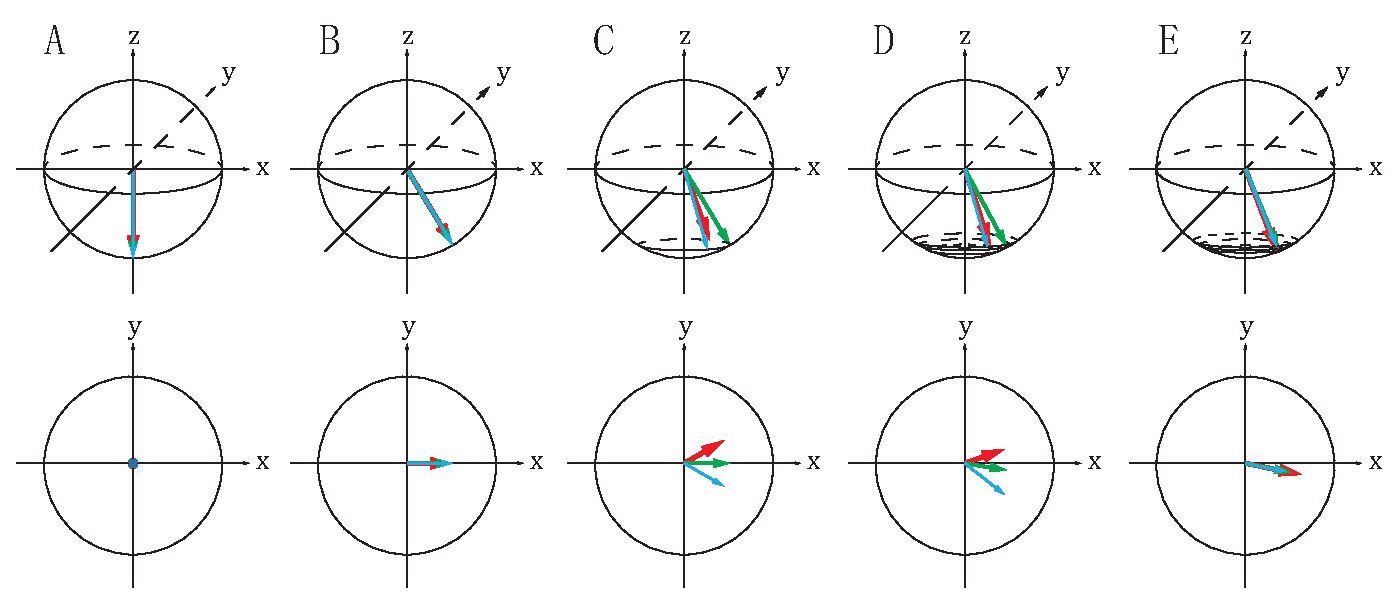
\includegraphics[width=1.0\textwidth]{1.eps}
            \caption{The evolution of different sub-ensembles on Bloch sphere. The lower figures are corresponding plan views from positive $z$ direction.}
            \label{B-S}
        \end{figure}

        \textbf{A}: Before the pulses, any certain ensemble's Bloch vector is at their equilibrium state. Since their density matrix have only the diagonal elements, the Bloch vector of all the ensembles only have $z$ component, and are along the negative $z$ direction on the Bloch sphere.\\
        \textbf{B}: Tipped by the first pulse, say, the Bloch vectors of all the ensembles rotate about the $y$ axis by a small angle ($\theta=\int R_1(t)dt$).\\
        \textbf{C}: Since different ensembles have different resonant frequencies, their Bloch vectors dephase and the length of the sum of their projections on the $xy$ plane (and thus the polarization of the system) will decay. More specifically, the red Bloch vector corresponding to a greater resonant frequency (i.e., greater pseudo magnetic field, see equation \ref{PMF-2}) rotates through a greater angle, while the blue Bloch vector corresponding to a smaller resonant frequency rotate through a smaller angle during the evolution between the two pulse. The green Bloch vector is of an average resonant frequency. (In plan view, it is just a coincidence that the green Bloch's projection on $xy$ plane rotates to along $x$ direction at $T$, it does not have to.)\\
        \textbf{D}: Suppose the second pulse rotates all the Bloch vectors, say, about the $x$ axis clockwisely for small angle ($\theta=\int R_2(t)dt$). We find that the faster-rotating (red) Bloch vector's projection on the $xy$ plane is lengthened, while the slower-rotating Bloch (blue) vector's projection is shortened. In this way, the rotating frequency of the red Bloch vector is slowed down while the rotating frequency of the blue Bloch vector becomes more faster after the second pulse.\\
        \textbf{E}: $T$ after the second pulse, the blue Bloch vector's projection on $xy$ plane will catch up the red Bloch's projection on $xy$. The sum of all the ensemble's Bloch vectors projections on $xy$ plane will reach a peak and this will cause an echo of polarization of the system.
        \item[(b)] We use $\lvert 0\rangle$ to represent for the ground state of an atom and $\lvert 1\rangle$ for the upper state. Suppose before the input of the pulses (which means, at equilibrium), the density operator of the system is
        \begin{equation}
            \hat{\rho}^0=\rho_{00}^0\lvert 0\rangle\langle 0\rvert+\rho_{11}^0\lvert 1\rangle\langle 1\rvert,
        \end{equation}
        so the Bloch vector of the initial state is
        \begin{equation}
            \vec{u}^0=(0,0,\rho_{11}^0-\rho_{00}^0).
        \end{equation}
        The pseudo magnetic field is
        \begin{align}
            \nonumber\vec{\Omega}=&(2\re{\vec{\mu}_{10}\cdot[\vec{E}_1(t)+\vec{E}_2(t)]/\hbar},-2\im{\vec{u}_{10}\cdot[\vec{E}_1(t)+\vec{E}_2(t)]/\hbar},-\omega_{10})\\
            =&(2\re{R_1(t)+R_2(t)},-2\im{R_1(t)+R_2(t)},-\omega_{10}).
        \end{align}
        The equation of motion of $\vec{u}$ is
        \begin{equation}
            \label{ME}
            \frac{d}{dt}\vec{u}=\vec{u}\times\vec{\Omega}.
        \end{equation}
        Integrating the above equation from the initial, $-\infty$, to the moment right after the first pulse, $0^+$, we get
        \begin{equation}
            \vec{u}(0^+)-\vec{u}^0=\int_{-\infty}^{0^+}\frac{d}{dt}\vec{u}=\int_{-\infty}^{0^+}dt\,\vec{u}(t)\times\vec{\Omega}=\vec{u}^0\times\left[\begin{matrix}
                2\re{\int R_1(\tau)\,dt}\\
                -2\im{\int R_1(\tau)\,dt}\\
                -\omega_{10}
            \end{matrix}\right]=\left[\begin{matrix}
                2\im{\int R_1(\tau)\,d\tau}(\rho_{11}^0-\rho_{00}^0)\\
                2\re{\int R_1(\tau)\,d\tau}(\rho_{11}^0-\rho_{00}^0)\\
                0
            \end{matrix}\right],
        \end{equation}
        so the Bloch vector right after the first pulse is
        \begin{equation}
            \label{BV-2}
            \vec{u}(0^+)=\left[\begin{matrix}
                2\im{\int R_1(\tau)\,d\tau}(\rho_{11}^0-\rho_{00}^0)\\
                2\re{\int R_1(\tau)\,d\tau}(\rho_{11}^0-\rho_{00}^0)\\
                \rho_{11}^0-\rho_{00}^0
            \end{matrix}\right].
        \end{equation}
        Between the first and the second pulses, the pseudo magnetic field is along the negative $z$ direction:
        \begin{equation}
            \label{PMF-2}
            \vec{\Omega}'=(0,0,-\omega_{10}),
        \end{equation}
        but the pseudo Bloch vector has some components perpendicular to $z$ axis, so it will rotate about the $z$ axis. The equation of motion is
        \begin{equation}
            \frac{d}{dt}\left[\begin{matrix}
                2\re{\rho_{10}(t)}\\
                -2\im{\rho_{10}(t)}\\
                \rho_{11}(t)-\rho_{00}(t)
            \end{matrix}\right]=\frac{d}{dt}\vec{u}(t)=\vec{u}(t)\times\vec{\Omega}(t)=\left[\begin{matrix}
                2\im{\rho_{10}(t)}\omega_{10}\\
                2\re{\rho_{10}(t)}\omega_{10}\\
                0
            \end{matrix}\right].
        \end{equation}
        Solving the above motion equation and using equation \eqref{BV-2}, we get
        \begin{align}
            \vec{u}(t)=\left[\begin{matrix}
                -2\im{\int R_1^*(\tau)\,d\tau\,e^{i\omega_{10}t}}(\rho_{11}^0-\rho_{00}^0)\\
                2\re{\int R_1^*(\tau)\,d\tau\,e^{i\omega_{10}t}}(\rho_{11}^0-\rho_{00}^0)\\
                \rho_{11}^0-\rho_{00}^0
            \end{matrix}\right].
        \end{align}
        Actually, the system consists of different ensembles with different resonant frequencies and the Bloch vector above is only of the ensemble with the resonant frequencies $\omega_{10}$. They will rotate about $z$ axis with slightly different frequencies and cause dephasing. We set the dephasing time to be $T_2^*=\frac{1}{\Gamma_2}$. The expectation of the Bloch vector between the two pulse is
        \begin{equation}
            \langle\vec{u}(t)\rangle=\left[\begin{matrix}
                -2\im{\int R_1^*(\tau)\,d\tau\,e^{i(\omega_{10}+i\Gamma_2)t}}(\rho_{11}^0-\rho_{00}^0)\\
                2\re{\int R_1^*(\tau)\,d\tau\,e^{i(\omega_{10}+i\Gamma_2)t}}(\rho_{11}^0-\rho_{00}^0)\\
                \rho_{11}^0-\rho_{00}^0
            \end{matrix}\right].
        \end{equation}
        The expectation of the Bloch vector right before the second pulse is
        \begin{equation}
            \langle\vec{u}(T^-)\rangle=\left[\begin{matrix}
                -2\im{\int R_1^*(\tau)\,d\tau\,e^{i(\omega_{10}+i\Gamma_2)T}}(\rho_{11}^0-\rho_{00}^0)\\
                2\re{\int R_1^*(\tau)\,d\tau\,e^{i(\omega_{10}+i\Gamma_2)T}}(\rho_{11}^0-\rho_{00}^0)\\
                \rho_{11}^0-\rho_{00}^0
            \end{matrix}\right].
        \end{equation}
        Integrating the equation of motion from the moment right before the second pulse, $T^-$ to the moment right after the second pulse, we get
        \begin{equation}
            \langle\vec{u}(T^+)\rangle-\langle\vec{u}(T^-)\rangle=\int_{T^-}^{T^+}dt\,\frac{d}{dt}\langle\vec{u}(t)\rangle=\int_{T^-}^{T^+}dt\,\langle\vec{u}\rangle\times\vec{\Omega}=\left[\begin{matrix}
                2\im{\int R_2(\tau)\,d\tau}(\rho_{11}^0-\rho_{00}^0)\\
                2\re{\int R_2(\tau)\,d\tau}(\rho_{11}^0-\rho_{00}^0)\\
                0
            \end{matrix}\right],
        \end{equation}
        so the Bloch vector right after the second pulse is
        \begin{equation}
            \label{BV-4}
            \langle\vec{u}(T^+)\rangle=\left[\begin{matrix}
                -2\im{\int R_1^*(\tau)\,d\tau\,e^{i(\omega_{10}+i\Gamma_{10})T}-\int R_2(\tau)\,d\tau}(\rho_{11}^0-\rho_{00}^0)\\
                2\re{\int R_1^*(\tau)\,d\tau\,e^{i(\omega_{10}+i\Gamma_{10})T}+\int R_2(\tau)\,d\tau}(\rho_{11}^0-\rho_{00}^0)\\
                \rho_{11}^0-\rho_{00}^0
            \end{matrix}\right]
        \end{equation}
        After the second pulse, the pseudo magnetic field is again
        \begin{equation}
            \vec{\Omega}'=(0,0,-\omega_{10}),
        \end{equation}
        and equation of motion is again
        \begin{equation}
            \frac{d}{dt}\left[\begin{matrix}
                2\re{\rho_{10}(t)}\\
                -2\im{\rho_{10}(t)}\\
                \rho_{11}(t)-\rho(t)
            \end{matrix}\right]=\frac{d}{dt}\vec{u}(t)=\vec{u}(t)\times\vec{\Omega}(t)=\left[\begin{matrix}
                2\im{\rho_{10}(t)}\omega_{10}\\
                2\re{\rho_{10}(t)}\omega_{10}\\
                0
            \end{matrix}\right].
        \end{equation}
        Solving the equation of motion and using equation \eqref{BV-4}, we get the Bloch vector at time $T+t$:
        \begin{equation}
            \vec{u}(T+t)=\left[\begin{matrix}
                2\im{[\int R_1(\tau)\,d\tau\,e^{-i(\omega_{10}+i\Gamma_2)T}-\int R_2^*(\tau)\,d\tau]e^{i\omega_{10}t}}(\rho_{11}^0-\rho_{00}^0)\\
                2\re{[\int R_1(\tau)\,d\tau\,e^{-i(\omega_{10}+i\Gamma_2)T}+\int R_2^*(\tau)\,d\tau]e^{i\omega_{10}t}}(\rho_{11}^0-\rho_{00}^0)\\
                \rho_{11}^0-\rho_{00}^0
            \end{matrix}\right].
        \end{equation}
        Taking the dephasing effect into consideration, we have the expectation of the Bloch vector:
        \begin{equation}
            \langle\vec{u}(T+t)\rangle=\left[\begin{matrix}
                2\im{[\int R_1(\tau)\,d\tau\,e^{-i(\omega_{10}+i\Gamma_2)T}-\int R_2^*(\tau)\,d\tau]e^{i(\omega_{10}+i\Gamma_2)t}}(\rho_{11}^0-\rho_{00}^0)\\
                2\re{[\int R_1(\tau)\,d\tau\,e^{-i(\omega_{10}+i\Gamma_2)T}+\int R_2^*(\tau)\,d\tau]e^{i(\omega_{10}+i\Gamma_2)t}}(\rho_{11}^0-\rho_{00}^0)\\
                \rho_{11}^0-\rho_{00}^0
            \end{matrix}\right].
        \end{equation}
        At time $2T$, the Bloch vector is
        \begin{equation}
            \vec{u}(2T)=\left[\begin{matrix}
                2\im{[\int R_1(\tau)\,d\tau\,e^{-i(\omega_{10}+i\Gamma_{10})T}-\int R_2^*(\tau)\,d\tau]e^{i(\omega_{10}+i\Gamma_2)T}}(\rho_{11}^0-\rho_{00}^0)\\
                2\re{[\int R_1(\tau)\,d\tau\,e^{-i(\omega_{10}+i\Gamma_{10})T}+\int R_2^*(\tau)\,d\tau]e^{i(\omega_{10}+i\Gamma_2)T}}(\rho_{11}^0-\rho_{00}^0)\\
                \rho_{11}^0-\rho_{00}^0
            \end{matrix}\right]\equiv\left[\begin{matrix}
                2\re{\rho_{10}(2T)}\\
                -2\im{\rho_{10}(2T)}\\
                \rho_{11}(2T)-\rho_{00}(2T)
            \end{matrix}\right],
        \end{equation}
        so the coherence element of the density matrix of the system at time $2T$ is
        \begin{align}
            \nonumber\langle\rho_{10}(2T)\rangle=&\left\{\im{\int R_1(\tau)\,d\tau-\int R_2^*(\tau)\,d\tau\,e^{i(\omega_{10}+i\Gamma_2)T}}-i\re{\int R_1(\tau)\,d\tau+\int R_2^*(\tau)\,d\tau\,e^{i(\omega_{10}t+i\Gamma_2)T}}\right\}(\rho_{11}^0-\rho_{00}^0)\\
            =&-i\left[\int R_1(\tau)\,d\tau+\int R_2(\tau)\,d\tau\,e^{-i(\omega_{10}+i\Gamma_2)T}\right](\rho_{11}^0-\rho_{00}^0).
        \end{align}
        The polarization of the system at time $2T$ is
        \begin{align}
            \nonumber\rho_{10}(2T)=&\text{Tr}(N\vec{u}\rho(2T))=N[\mu_{10}\rho_{01}(2T)+\mu_{01}\rho_{10}(2T)]=2N\re{\mu_{01}\rho_{10}(2T)}\\
            =&2N\re{-i\mu_{01}\left[\int R_1(\tau)\,d\tau+\int R_2(\tau)\,d\tau\,e^{-i(\omega_{10}+i\Gamma_2)T}\right](\rho_{11}^0-\rho_{00}^0)}\\
            =&2N\im{\mu_{01}\left[\int R_1(\tau)\,d\tau+\int R_2(\tau)\,d\tau\,e^{-i(\omega_{10}+i\Gamma_2)T}\right](\rho_{11}^0-\rho_{00}^0)}.
        \end{align}
    \end{enumerate}
\end{sol}
\end{document}